
\documentclass[letterpaper,hide notes,xcolor={table,svgnames},pdftex,10pt]{beamer}
\def\showexamples{t}

\usecolortheme{crane}
\setbeamertemplate{navigation symbols}{}

\usetheme{MyPittsburgh}
\usepackage{hyperref}
\usepackage{graphicx,xspace}
\usepackage[normalem]{ulem}
\usepackage{multicol}
\usepackage{amsmath,amssymb,amsthm,graphicx,xspace}
\newcommand\SF[1]{$\bigstar$\footnote{SF: #1}}

\usepackage[sfdefault,lf]{carlito}
\usepackage[T1]{fontenc}
\usepackage[scaled]{beramono}
\usepackage{tikzpagenodes}
\newcommand{\Rplus}{\protect\hspace{-.1em}\protect\raisebox{.35ex}{\small{\small\textbf{+}}}}
\newcommand{\Cpp}{\mbox{C\Rplus\Rplus}\xspace}

\newcounter{tmpnumSlide}
\newcounter{tmpnumNote}

\newcommand\mnote[1]{%
	\addtocounter{tmpnumSlide}{1}
	\ifdefined\showcues {~\tiny\fbox{\arabic{tmpnumSlide}}}\fi
	\note{\setlength{\parskip}{1ex}\addtocounter{tmpnumNote}{1}\textbf{\Large \arabic{tmpnumNote}:} {#1\par}}}

\newcommand\mmnote[1]{\note{\setlength{\parskip}{1ex}#1\par}}


\newcommand\mquestion[2]{{~\color{red}\fbox{?}}\note{\setlength{\parskip}{1ex}\par{\Large \textbf{?}} #1} \note{\setlength{\parskip}{1ex}\par{\Large \textbf{A}} #2\par}\ifdefined \presentationonly \pause \fi}

\newcommand\blackboard[1]{%
	\ifdefined   \showblackboard
		{#1}
	\else {\begin{center} \fbox{\colorbox{blue!30}{%
						\begin{minipage}{.95\linewidth}%
							\hspace{\stretch{1}} Some space intentionally left blank; done at the blackboard.%
						\end{minipage}}}\end{center}}%
	\fi%
}

\usepackage{listings}
\lstset{%
	keywordstyle=\bfseries,
	aboveskip=15pt,
	belowskip=15pt,
	captionpos=b,
	identifierstyle=\ttfamily,
	frame=lines,
	numbers=left, basicstyle=\scriptsize, numberstyle=\tiny, stepnumber=0, numbersep=2pt}

\usepackage{siunitx}
\newcommand\sius[1]{\num[group-separator = {,}]{#1}\si{\micro\second}}
\newcommand\sims[1]{\num[group-separator = {,}]{#1}\si{\milli\second}}
\newcommand\sins[1]{\num[group-separator = {,}]{#1}\si{\nano\second}}
\sisetup{group-separator = {,}, group-digits = true}

%% -------------------- tikz --------------------
\usepackage{tikz}
\usetikzlibrary{positioning}
\usetikzlibrary{arrows,backgrounds,automata,decorations.shapes,decorations.pathmorphing,decorations.markings,decorations.text}

\tikzstyle{place}=[circle,draw=blue!50,fill=blue!20,thick, inner sep=0pt,minimum size=6mm]
\tikzstyle{transition}=[rectangle,draw=black!50,fill=black!20,thick, inner sep=0pt,minimum size=4mm]

\tikzstyle{block}=[rectangle,draw=black, thick, inner sep=5pt]
\tikzstyle{bullet}=[circle,draw=black, fill=black, thin, inner sep=2pt]

\tikzstyle{pre}=[<-,shorten <=1pt,>=stealth',semithick]
\tikzstyle{post}=[->,shorten >=1pt,>=stealth',semithick]
\tikzstyle{bi}=[<->,shorten >=1pt,shorten <=1pt, >=stealth',semithick]

\tikzstyle{mut}=[-,>=stealth',semithick]

\tikzstyle{treereset}=[dashed,->, shorten >=1pt,>=stealth',thin]

\usepackage{ifmtarg}
\usepackage{xifthen}
\makeatletter
% new counter to now which frame it is within the sequence
\newcounter{multiframecounter}
% initialize buffer for previously used frame title
\gdef\lastframetitle{\textit{undefined}}
% new environment for a multi-frame
\newenvironment{multiframe}[1][]{%
	\ifthenelse{\isempty{#1}}{%
		% if no frame title was set via optional parameter,
		% only increase sequence counter by 1
		\addtocounter{multiframecounter}{1}%
	}{%
		% new frame title has been provided, thus
		% reset sequence counter to 1 and buffer frame title for later use
		\setcounter{multiframecounter}{1}%
		\gdef\lastframetitle{#1}%
	}%
	% start conventional frame environment and
	% automatically set frame title followed by sequence counter
	\begin{frame}%
		\frametitle{\lastframetitle~{\normalfont(\arabic{multiframecounter})}}%
		}{%
	\end{frame}%
}
\makeatother

\makeatletter
\newdimen\tu@tmpa%
\newdimen\ydiffl%
\newdimen\xdiffl%
\newcommand\ydiff[2]{%
	\coordinate (tmpnamea) at (#1);%
	\coordinate (tmpnameb) at (#2);%
	\pgfextracty{\tu@tmpa}{\pgfpointanchor{tmpnamea}{center}}%
	\pgfextracty{\ydiffl}{\pgfpointanchor{tmpnameb}{center}}%
	\advance\ydiffl by -\tu@tmpa%
}
\newcommand\xdiff[2]{%
	\coordinate (tmpnamea) at (#1);%
	\coordinate (tmpnameb) at (#2);%
	\pgfextractx{\tu@tmpa}{\pgfpointanchor{tmpnamea}{center}}%
	\pgfextractx{\xdiffl}{\pgfpointanchor{tmpnameb}{center}}%
	\advance\xdiffl by -\tu@tmpa%
}
\makeatother
\newcommand{\copyrightbox}[3][r]{%
	\begin{tikzpicture}%
		\node[inner sep=0pt,minimum size=2em](ciimage){#2};
		\usefont{OT1}{phv}{n}{n}\fontsize{4}{4}\selectfont
		\ydiff{ciimage.south}{ciimage.north}
		\xdiff{ciimage.west}{ciimage.east}
		\ifthenelse{\equal{#1}{r}}{%
			\node[inner sep=0pt,right=1ex of ciimage.south east,anchor=north west,rotate=90]%
			{\raggedleft\color{black!50}\parbox{\the\ydiffl}{\raggedright{}#3}};%
		}{%
			\ifthenelse{\equal{#1}{l}}{%
				\node[inner sep=0pt,right=1ex of ciimage.south west,anchor=south west,rotate=90]%
				{\raggedleft\color{black!50}\parbox{\the\ydiffl}{\raggedright{}#3}};%
			}{%
				\node[inner sep=0pt,below=1ex of ciimage.south west,anchor=north west]%
				{\raggedleft\color{black!50}\parbox{\the\xdiffl}{\raggedright{}#3}};%
			}
		}
	\end{tikzpicture}
}


%% --------------------

%\usepackage[excludeor]{everyhook}
%\PushPreHook{par}{\setbox0=\lastbox\llap{MUH}}\box0}

%\vspace*{\stretch{1}

%\setbox0=\lastbox \llap{\textbullet\enskip}\box0}

\setlength{\parskip}{\fill}

\newcommand\noskips{\setlength{\parskip}{1ex}}
\newcommand\doskips{\setlength{\parskip}{\fill}}

\newcommand\xx{\par\vspace*{\stretch{1}}\par}
\newcommand\xxs{\par\vspace*{2ex}\par}
\newcommand\tuple[1]{\langle #1 \rangle}
\newcommand\code[1]{{\sf \footnotesize #1}}
\newcommand\ex[1]{\uline{Example:} \ifdefined \presentationonly \pause \fi
	\ifdefined\showexamples#1\xspace\else{\uline{\hspace*{2cm}}}\fi}

\newcommand\ceil[1]{\lceil #1 \rceil}


\AtBeginSection[]
{
	\begin{frame}
		\frametitle{Outline}
		\tableofcontents[currentsection]
	\end{frame}
}



\pgfdeclarelayer{edgelayer}
\pgfdeclarelayer{nodelayer}
\pgfsetlayers{edgelayer,nodelayer,main}

\tikzstyle{none}=[inner sep=0pt]
\tikzstyle{rn}=[circle,fill=Red,draw=Black,line width=0.8 pt]
\tikzstyle{gn}=[circle,fill=Lime,draw=Black,line width=0.8 pt]
\tikzstyle{yn}=[circle,fill=Yellow,draw=Black,line width=0.8 pt]
\tikzstyle{empty}=[circle,fill=White,draw=Black]
\tikzstyle{bw} = [rectangle, draw, fill=blue!20,
text width=4em, text centered, rounded corners, minimum height=2em]

\newcommand{\CcNote}[1]{% longname
	This work is licensed under the \textit{Creative Commons #1 3.0 License}.%
}
\newcommand{\CcImageBy}[1]{%
	\includegraphics[scale=#1]{creative_commons/cc_by_30.pdf}%
}
\newcommand{\CcImageSa}[1]{%
	\includegraphics[scale=#1]{creative_commons/cc_sa_30.pdf}%
}
\newcommand{\CcImageNc}[1]{%
	\includegraphics[scale=#1]{creative_commons/cc_nc_30.pdf}%
}
\newcommand{\CcGroupBySa}[2]{% zoom, gap
	\CcImageBy{#1}\hspace*{#2}\CcImageNc{#1}\hspace*{#2}\CcImageSa{#1}%
}
\newcommand{\CcLongnameByNcSa}{Attribution-NonCommercial-ShareAlike}

\newenvironment{changemargin}[1]{% 
	\begin{list}{}{% 
		\setlength{\topsep}{0pt}% 
		\setlength{\leftmargin}{#1}% 
		\setlength{\rightmargin}{1em}
		\setlength{\listparindent}{\parindent}% 
		\setlength{\itemindent}{\parindent}% 
		      \setlength{\parsep}{\parskip}% 
		      }% 
		\item[]}{\end{list}}




\title{Lecture 8 --- The Heap: Dynamic Memory Allocation}

\author{Jeff Zarnett \\ \small \texttt{jzarnett@uwaterloo.ca}}
\institute{Department of Electrical and Computer Engineering \\
  University of Waterloo}
\date{\today}


\begin{document}

\begin{frame}
  \titlepage

 \end{frame}
 
 
\begin{frame}
\frametitle{Dynamic Memory Allocation}
 
 \begin{center}
	
\includegraphics[width=0.7\textwidth]{images/chrome.jpg}
\end{center}

\end{frame}

\begin{frame}
\frametitle{Dynamic Memory Allocation}

What's the heap? It's a large, programmer-managed memory region.

It's where \alert{dynamic} (run-time) memory allocation happens.

\end{frame}

\begin{frame}
\frametitle{General Memory Allocation Interface}

C works on memory with: \texttt{malloc()} and \texttt{free()}. 

This level is a lot closer to the way the operating system thinks about memory: \\
\quad Tell me how much you need and tell me when you are finished with it.

Other languages implement garbage collection or other strategies.

\end{frame}

\begin{frame}
\frametitle{Using Memory Allocation in C}

To allocate an integer, you call \texttt{malloc( sizeof( int ) )}. 

This creates, somewhere in memory, a new integer and returns the address of it that can be stored in a pointer.

To be sure to ask for the correct amount of memory, we have \texttt{sizeof} which works out the size of its argument (integer).


\end{frame}

\begin{frame}
\frametitle{Using Memory Deallocation in C}

When you \texttt{free()} that pointer, the memory is marked as available.

It is not necessarily cleared or reused right away.

\end{frame}

\begin{frame}
\frametitle{Using Memory Deallocation in C}

This is why you can sometimes get away with dereferencing a pointer after it has been freed. 

\begin{center}
	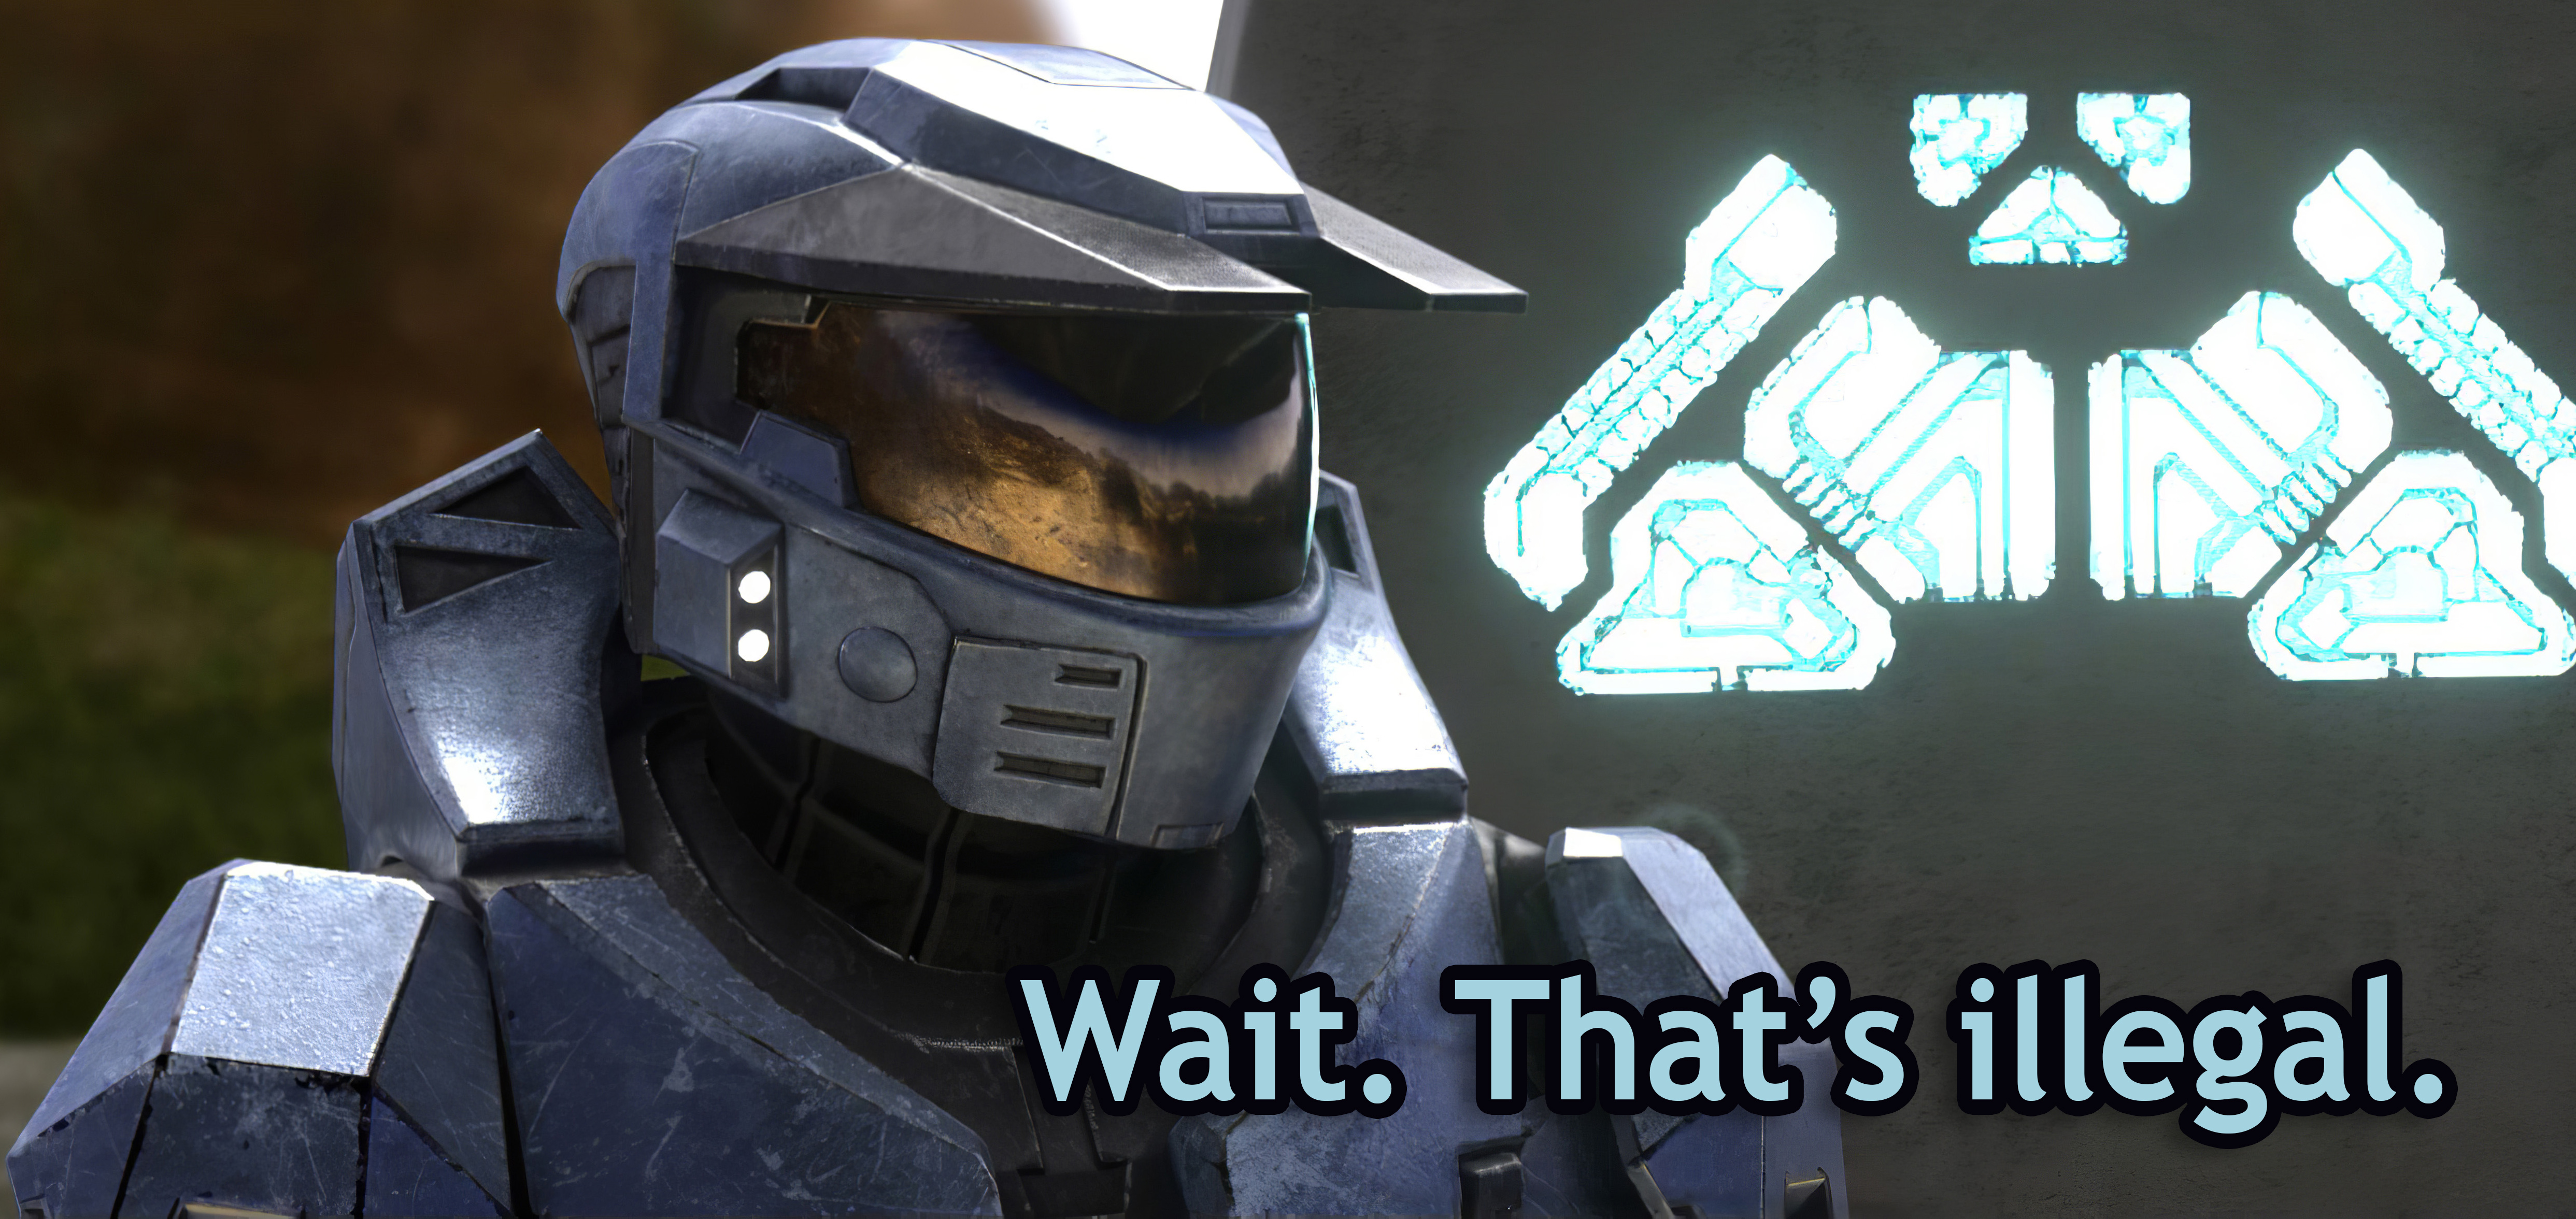
\includegraphics[width=0.8\textwidth]{images/illegal.jpg}
\end{center}

Sometimes it takes a while for that memory to be reclaimed or reused so the old value just happens to still be there in memory. 

\end{frame}

\begin{frame}
\frametitle{Returning Memory when Done}

Note that \texttt{free()} does not specify how much memory is being returned. 

This means two things:\\ 
\quad (1) that the operating system is keeping track of each allocated block's size\\
\quad (2) that it is not possible to return part of a block.

\end{frame}

\begin{frame}
\frametitle{Leak}

But remember: you have to explicitly deallocate it...\\
\quad Otherwise we have a \alert{memory leak}.

Memory leaks are a huge problem in programming...

\end{frame}

\begin{frame}
\frametitle{Fulfilling Memory Requests}

The operating system will try to find some free memory to meet the request. 

Running out of memory is a rare thing given the size of main memory in a modern computer.

There is still the possibility that some request may not be fulfilled because no block meeting that need is available.

\end{frame}


\begin{frame}
\frametitle{Arranging Blocks}

Let's consider how to arrange the blocks...

\begin{center}
	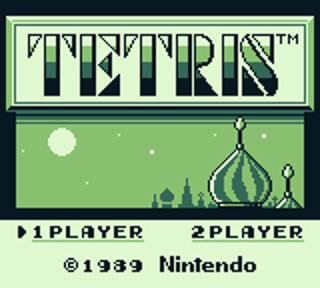
\includegraphics[width=0.4\textwidth]{images/Tetris01.png}
	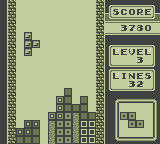
\includegraphics[width=0.4\textwidth]{images/Tetris02.png}
\end{center}


\end{frame}


\begin{frame}
\frametitle{Fixed Block Sizes}

One possibility for how to allocate memory is in fixed block sizes. 

All blocks of memory allocated are the same size. 

If a request comes in for 1 byte, 1 block is allocated. 

If a request comes in that is, say, 1.5 blocks, 2 blocks are allocated. 


\end{frame}

\begin{frame}
\frametitle{Fixed Block Sizes: Wasteful?}

It is immediately obvious when we look at this that some memory is ``wasted''. 

If 1.5 blocks are requested and 2 blocks are allocated and returned, we are using up an extra 0.5 blocks. 

This space cannot be used for anything useful (as it shows as allocated).

\end{frame}

\begin{frame}
\frametitle{Fixed Block Sizes: Wasteful?} 

This is a problem called \alert{internal fragmentation}.

The bigger each block is, the more memory will be wasted.


\end{frame}

\begin{frame}
\frametitle{Fixed: One Size of Blocks}

Suppose the system has only one size of blocks, perhaps, 1~KB. 

\begin{center}
	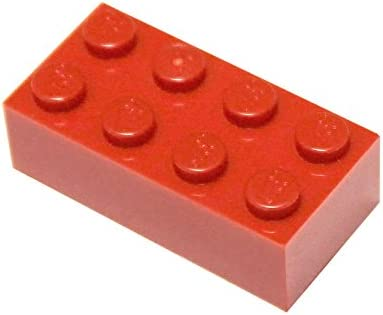
\includegraphics[width=0.3\textwidth]{images/lego.jpg}
\end{center}

Divide up memory into blocks of this fixed size and maintain a linked list of addresses of all currently available blocks. 

\end{frame}

\begin{frame}
\frametitle{Fixed: One Size of Blocks}


When a block is allocated, remove its corresponding node from the linked list. 

When a block is freed, put a node with that address into the linked list. 

If the list is empty, a memory request cannot be satisfied; return null.

This is definitely fast as we can allocate memory in $\Theta(1)$ time.


\end{frame}

\begin{frame}
\frametitle{Fixed: Multiple Sizes}

Recognizing that some memory allocation requests are bigger than others, it might make sense to have several different block sizes.

\begin{center}
	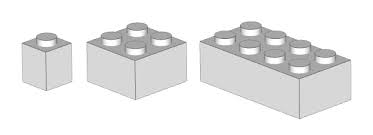
\includegraphics[width=0.5\textwidth]{images/lego3.jpg}
\end{center}

Perhaps 1~KB, 2~KB, and 4~KB. 

These can generally be allocated and deallocated in $\Theta(1)$ time if we have one linked list for each different size of block.


\end{frame}



\begin{frame}
\frametitle{Fixed: Fragmentation}

Unfortunately, fixed block sizes suffer from a lot of internal fragmentation. 

This may be suitable for embedded systems where simplicity and speed of operations are more important than worrying about wasting memory. 

This is, we can see, not how \texttt{malloc()} works.\\
\quad 1~KB of memory is not allocated to store a 4-byte integer. 
 
What we need instead is a variable block size.


\end{frame}


\begin{frame}
\frametitle{Variable Block Sizes}

\begin{center}
	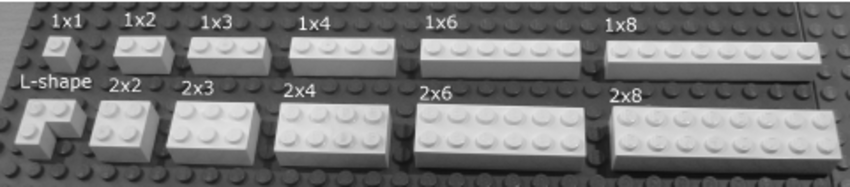
\includegraphics[width=\textwidth]{images/lego2.png}
\end{center}


\end{frame}


\begin{frame}
\frametitle{Variable Block Sizes}

Variable block sizes are not that different from fixed block sizes.

We just take the size of blocks down to the smallest they can be. 

In a system with byte-addressable memory, the smallest block is one byte.

Now a different problem: keeping track of what is allocated \& what is free.


\end{frame}

\begin{frame}
\frametitle{Variable: Bitmaps}

Divide memory into $M$ units of $n$ bits, and then to create a bit array of size $M$ storing the status of each of those units. 

If a bit $m$ in $M$ is 0, it means that unit is unallocated.\\
If it is 1 then that unit is allocated. 

\end{frame}

\begin{frame}
\frametitle{Variable: Bitmaps}


How much memory is lost to this overhead?\\
\quad $100/(n+1)$\% of the memory is used. 

If a unit is 4 bytes, the bitmap is about 3\% of memory; \\
If it is 16 bytes the bitmap takes about 0.8\% of memory. 

Finding a block of $k$ bytes requires searching the bitmap for a run of $\frac{8k}{n}$ zeros~.

\end{frame}

\begin{frame}
\frametitle{Variable: Linked Lists}

The other approach, as in the case of fixed size blocks, is to use linked lists. 

The info of the linked list can be stored separately from memory allocation.

Or it can be stored as part of the block of memory. Either approach is workable.

\end{frame}

\begin{frame}
\frametitle{Variable: Linked Lists}

After startup, the linked list contains one entry.\\
\quad  All available memory is in one contiguous block. 

When a memory request is allocated the block is divided up. 

Suppose we allocate the first 128 bytes.\\
\quad A new entry is placed in the list, at 128 bytes. 

The node that is added contains the start address, the length of the block, and a bit indicating it is allocated. 

\end{frame}

\begin{frame}
\frametitle{Variable: Linked Lists}

The unallocated block's node will contain the updated entry: smaller size, new start address, and the bit indicating it is unallocated. 

When a block is deallocated, we simply find that block in the linked list and set the bit to zero to indicate it is now available again.

\end{frame}


\begin{frame}
\frametitle{Efficiency Counts}
For a sufficiently-large memory area, one linked list is inefficient.

Why? May need to search all blocks and more allocations means more blocks.

Better idea: separate free block list!

\end{frame}


\begin{frame}
\frametitle{Variable: Deallocation}

In a typical system there may be a lot of allocation and deallocation of memory. 

This will probably lead to breaking memory up into smaller pieces.

We may end up with free blocks small and spread out:
\begin{center}
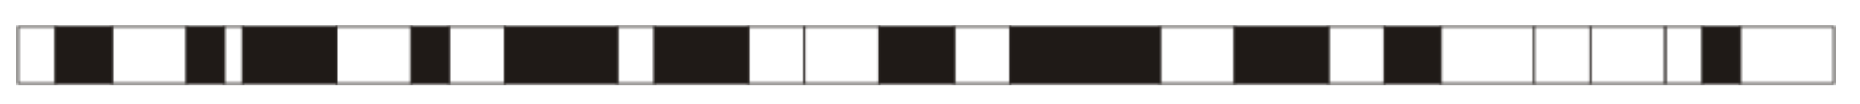
\includegraphics[width=0.9\textwidth]{images/checkerboard.png}
\end{center}



\end{frame}

\begin{frame}
\frametitle{Variable: Coalescence}

It may be that there is a contiguous block of free memory available of size $N$. 

A request for $N$ cannot be fulfilled because the memory is logically split up. 

To solve this, we need a way to recombine the split blocks; \alert{coalescence}:

\begin{center}
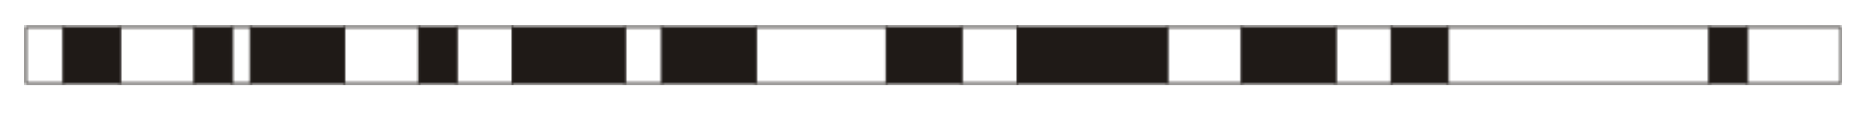
\includegraphics[width=0.9\textwidth]{images/checkerboard-coalesced.png}
\end{center}


\end{frame}

\begin{frame}
\frametitle{Coalescence}

Coalescence is just the process or merging two adjacent free blocks into one. 

Dividing memory should be a reversible operation. 

This solves the problem of $N$ contiguous bytes being unable to be allocated. 

Coalescence can be done periodically or whenever a block of memory is freed.


\end{frame}

\begin{frame}
\frametitle{Variable: Linked List \& Coalescence}

Coalescence makes it a good idea to maintain the memory blocks in a doubly-linked list.

When a block is freed, it may be in the middle of two free blocks. 

It is convenient to have previous and next pointers so the adjacent sections can be merged efficiently.


\end{frame}

\begin{frame}
\frametitle{Variable: External Fragmentation}

Even with coalescence, we may have the problem that $N$ free bytes exist in the system but spread out over many little pieces.

When free memory is spread into little tiny fragments, this situation is called \alert{external fragmentation}. 

It is analogous to internal fragmentation, except of course the tiny fragments are not inside any block.


\end{frame}

\begin{frame}
\frametitle{External Fragmentation}

One way to reduce external fragmentation is to increase internal fragmentation. 

If a request for $N$ bytes comes in and there is a block of $N+k$ available, where $k$ is very small, allocate the whole $N+k$ block for the request.

We just accept that $k$ bytes are lost to internal fragmentation.

\end{frame}

\begin{frame}
\frametitle{External Fragmentation Example}

If a free block contains 128 bytes and the request is for 120 bytes, it may not be worth the hassle and overhead to split this block into 120 and 8. 

Some systems round up memory allocations to the nearest power of 2 (e.g., a request for 28 bytes gets moved up to 32). 

Of course, this does not really help with satisfying the request for $N$ bytes of memory; it just keeps external fragmentation down.

\end{frame}

\begin{frame}
\frametitle{Memory Compaction}

Another idea is \alert{compaction}, which can also be thought of as \alert{relocation}. 

\begin{center}
	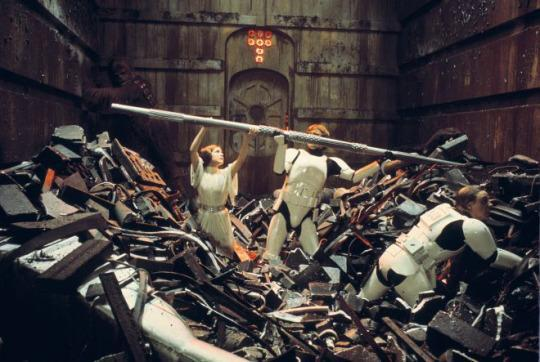
\includegraphics[width=0.5\textwidth]{images/compactor.jpg}
\end{center}

The goal is simply to move the allocated sections of memory next to one another in main memory, allowing for a large contiguous block of free space. 

\end{frame}

\begin{frame}
\frametitle{Memory Compaction}

This is a very expensive operation. 

The Java runtime, for example, must ``stop the world'' (halt all program execution) while it reorganizes memory. 

Even if we are willing to pay the cost, it might not be possible to do.

\end{frame}

\begin{frame}
\frametitle{Memory Compaction}

Languages with garbage collection like Java or C\# may do memory compaction as needed when the garbage collector runs.

This can work in such languages, because variables are references.

References can be moved around in memory at the garbage collector or runtime's convenience; all it needs to do is update every reference.

\end{frame}

\begin{frame}
\frametitle{Memory Compaction}


In C we operate directly on memory addresses. 

Thanks to things like pointer arithmetic and using integer variables as addresses, there is no reliable way to update all references.


\end{frame}

\begin{frame}
\frametitle{Variable: Allocation Strategies}

Given a memory request of $N$, where do we allocate the memory? 

\begin{center}
	\includegraphics[width=0.7\textwidth]{images/zoning.jpg}
\end{center}

\end{frame}

\begin{frame}
\frametitle{Variable: Allocation Strategies}

If there is no block of at least size $N$, the request cannot be satisfied. 

If there is only one, the decision is easy.

As long as memory has two free blocks of sufficient size ($N$ or more) that cannot be coalesced, a memory allocation request will require making a decision.


\end{frame}

\begin{frame}
\frametitle{Variable: Allocation Strategies}

We will examine the following strategies:

\begin{center}
	
\includegraphics[width=0.4\textwidth]{images/seuss.jpg}
\end{center}

\end{frame}

\begin{frame}
\frametitle{Variable: Allocation Strategies}

We will examine the following strategies:

\begin{enumerate}
	\item First fit.
	\item Next fit.
	\item Best fit.
	\item Worst fit.
	\item Quick fit.
\end{enumerate}

Let's use two linked lists: one for allocated memory and one for unallocated memory. 

\end{frame}

\begin{frame}
\frametitle{First Fit}

Start looking at the beginning of memory, and check each block. 

If the block is of sufficient size, split it to allocate the memory, and return the balance to the unallocated memory list. 

This algorithm has a runtime of $O(n)$ where $n$ is the number of blocks. 

This algorithm is simple to implement. 



\end{frame}

\begin{frame}
\frametitle{Next Fit}

Modification of first fit.

Keep track of where the last block was allocated, and then start the next search after that. 

This prevents the situation where there are a lot of small unallocated blocks (external fragmentation) all concentrated at the start of memory. 

The runtime is still $O(n)$, as with first fit.

\end{frame}



\begin{frame}
\frametitle{Best Fit}

We could instead try to make a more intelligent decision. 

Considering all blocks, we choose the smallest block that is at least as big as $N$.

This produces the smallest remaining unallocated space at the end. 

\end{frame}

\begin{frame}
\frametitle{Best Fit}

This would require either:\\
\quad (1) checking every available block ($\Theta(n)$ runtime); or\\
\quad (2) keeping the blocks sorted by increasing size ($O(n)$ runtime). 

If we use an AVL tree or red-black tree, then we can get best fit to run in $\Theta($ln$(n))$, possibly better runtime than first fit.

\end{frame}

\begin{frame}
\frametitle{Worst Fit}

The problem with best fit is that the leftover bits of memory are likely to be too small to be useful. 

Rather than trying to find the smallest block that is of size $N$ or greater, choose the largest block of free memory. 

When the block is split, the remaining free block is, hopefully, large enough to be useful. 



\end{frame}

\begin{frame}
\frametitle{Worst Fit}

As with best fit, we must either:\\
\quad (1) check each available block; or \\
\quad (2) keep the block sorted by size, though decreasing size this time. 

A max heap is appropriate, or a binomial or Fibonacci heap could also be appropriate.

\end{frame}

\begin{frame}
\frametitle{Quick Fit}

Though not a solution on its own, quick fit is an optimization. 

Use if memory requests of a certain size are known to be common. 

Common: requests for 1~MB.

Keep a separate list of blocks that are of perhaps 1-1.1~MB in size, so that if the request for 1~MB does come in, it can be satisfied immediately and quickly. 

\end{frame}

\begin{frame}
\frametitle{16 MB Allocation Example}

\begin{center}
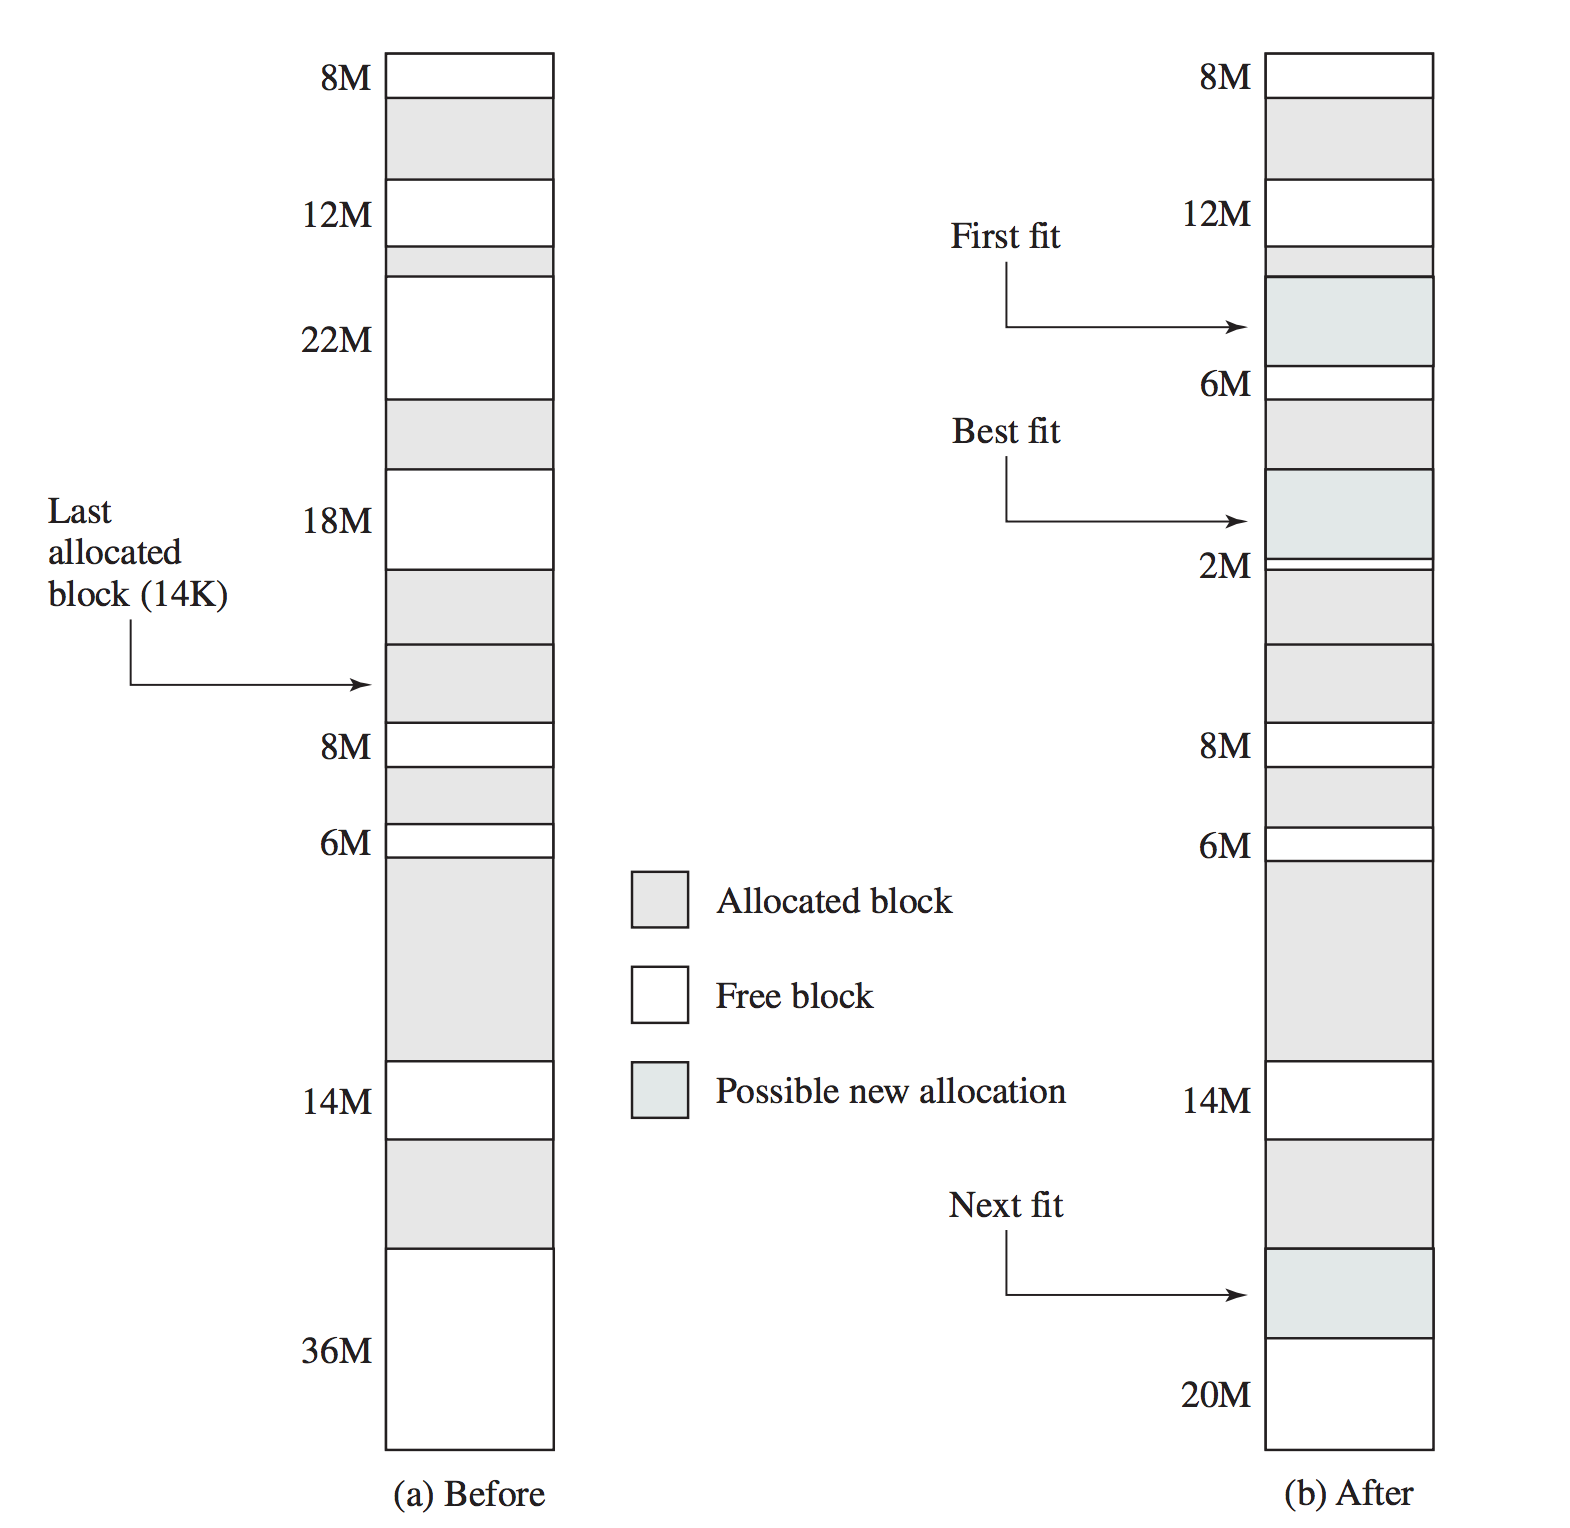
\includegraphics[width=0.60\textwidth]{images/first-best-next.png}
\end{center}


\end{frame}

\begin{frame}
\frametitle{Choosing a Strategy}

Simulations show that worst fit performs, well, worst in terms of time required to fulfill an allocation request and that it results in the most wasted space. 

First (next) and best fit are about equal in how well they utilize memory, but first fit tends to be faster. 

Despite this, even with optimization, given $x$ allocated blocks, another 0.5$x$ blocks may be lost to fragmentation.

\end{frame}



\begin{frame}
\frametitle{Choosing a Strategy}

The next fit algorithm tends to do allocations at the end of memory, so the largest block of free memory (typically at the end) is quickly broken up. 

First fit tends to litter the beginning of memory with small fragments.

Best fit tends to produce free blocks that are too small to be useful. 


\end{frame}



\begin{frame}
\frametitle{Binary Buddy}
How about a compromise between fixed and variable allocation?

There is some internal fragmentation, but it is a trade-off against how much external fragmentation we are willing to accept.

System: \alert{binary buddy}.


\end{frame}



\begin{frame}
\frametitle{Binary Buddy}

In a buddy system, memory blocks are available in powers of 2. 

More formally, a block is of size $2^{K}$, where $L \leq K \leq U$.

$2^{L}$ is the smallest block size that can be allocated.

$2^{U}$ is the largest block size that can be allocated (full size of memory). 

\end{frame}



\begin{frame}
\frametitle{Binary Buddy}

Initially, memory is treated as a single block of size $2^{U}$. 

If a request of size $n$ occurs, $2^{U-1} < n \leq 2^{U}$, then the entire block is allocated. 

Otherwise, the block is split into two ``buddies'', of size $2^{U-1}$. 

If $2^{U-2} < n \leq 2^{U-1}$, allocate one of the blocks of $2^{U-1}$ to the request.

Otherwise, subdivide again. 
 
Repeat until the smallest block greater than or equal to $n$ is allocated. 

\end{frame}

\begin{frame}
\frametitle{Binary Buddy}

In subsequent allocations, we look through the data structure to find either:\\
\quad (1) a block of appropriate size; or\\
\quad (2) a block that can be subdivided to meet the allocation. 

Whenever a pair of buddies (two blocks of equal size, split from the same ``parent'') in the list are both free, they can be coalesced.

\end{frame}


\begin{frame}
\frametitle{Binary Buddy 1~MB Block}

\begin{center}
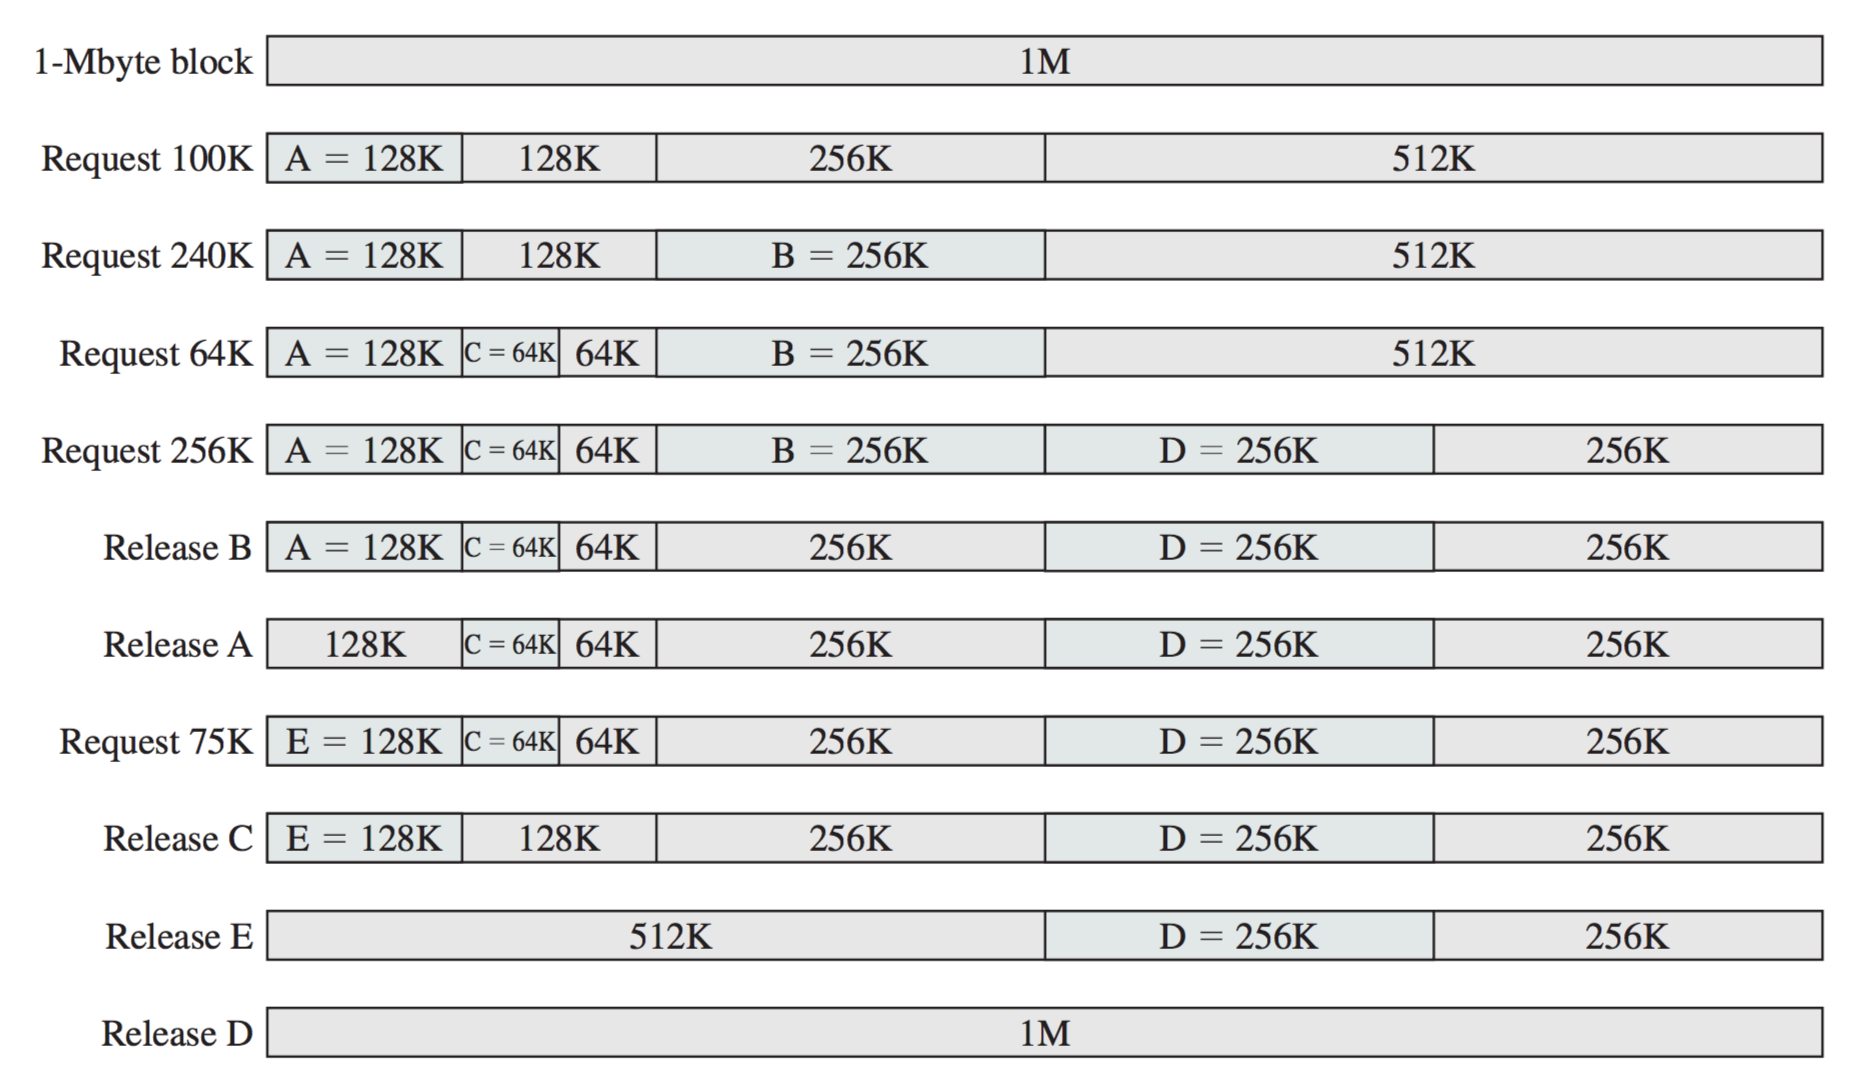
\includegraphics[width=\textwidth]{images/binary-buddy.png}
\end{center}


\end{frame}

\end{document}

